\subsection{Mezclador}
\paragraph{Mezclador}
El mezclador produce la resta y la suma de dos señales entrantes con distintas frecuencias. Si el dispositivo es de recepción, el mezclador normalmente se enfocará en obtener la resta entre la señal de RF y el oscilador local (LO). Si se encuentra en la etapa de transmisión, el mezclador normalmente producirá una señal RF muy superior en frecuencia a la señal de entrada con ayuda de un oscilador local con frecuencia mayor a la frecuencia de entrada IF.
\paragraph{Aislamiento entre puertos}
No se desean los componentes frecuenciales del oscilador local ni de la entrada en la salida o viceversa. Por esta razón los mezcladores al igual que los osciladores pueden ser balanceados o doblemente balanceados. Existen a su vez dos formas principales de implementar estos mezcladores: Mezclador con transistores y mezclador con diodos (y transformadores) En este trabajo se usaron dos mezcladores balanceados (balanceado simple) balanceado usando diodos shotcky 1N4148. 
\subsubsection{Diseño}
Para el diseño se debe considerar si se desea producir una 
\subsubsection{Simulación}
En la siguiente imagen se puede ver el esquema simulado en LTSpice. 
\begin{figure}
    \centering
    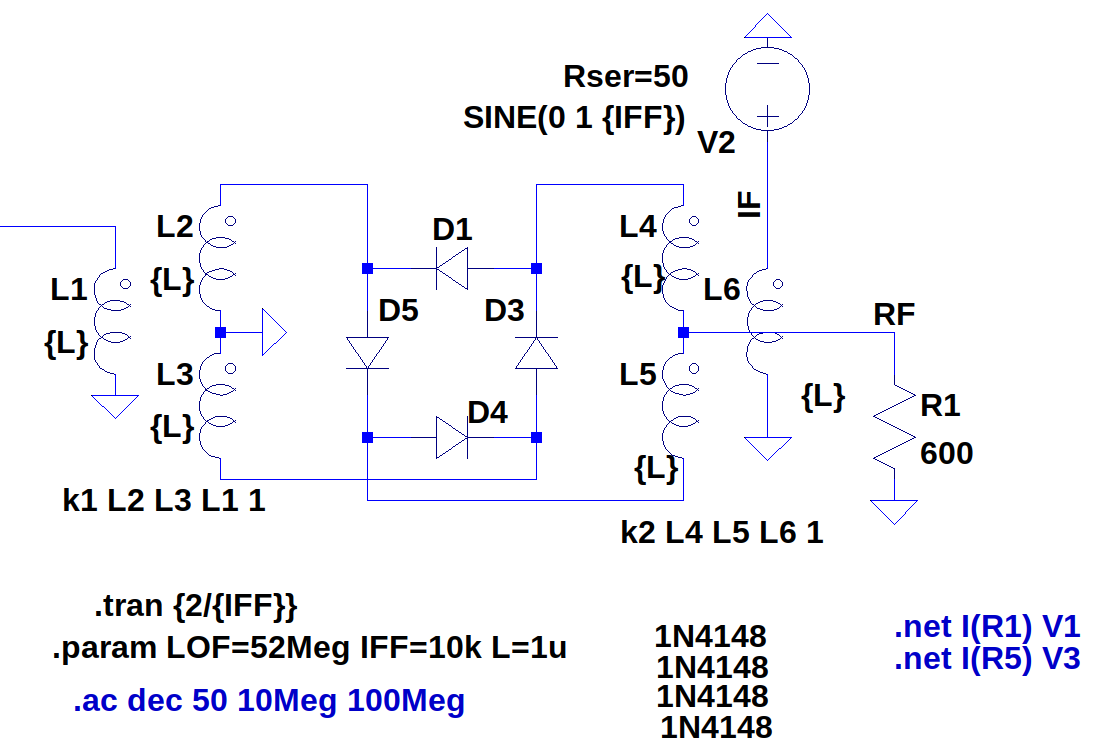
\includegraphics[width=0.5\linewidth]{Images/MIXERSIMU.png}
    \caption{Mezclador de diodos doblemente balanceado}
    \label{fig:mezDiod2}
\end{figure}